\documentclass{beamer}
\usetheme[background=light,block=fill,]{metropolis} % Use metropolis theme
% \usetheme{Madrid}
\usepackage{amsmath,amssymb,amsfonts,amsthm,mathtools}
\usepackage{enumitem}
\usepackage{xfrac}
\usepackage{hyperref}
\title{Classical Invariant Theory}
\subtitle{}
\date{April 22, 2024}
\author{Aryaman Maithani}
\institute{University of Utah}
\usepackage{parskip}

\usepackage[
	hyperref = true,      	% Link to online documents
  	backend  = bibtex,      % Use bibtex instead of biber
  	sorting  = nyt,       	% Sorts by (name, year, title)
  	% style  = alphabetic, 	% Citations look like [Har77]
  	maxbibnames = 5,
  	doi=false,isbn=false,url=false,eprint=false
]{biblatex}
\addbibresource{talks.bib}

\newcommand{\deff}[1]{{\color{blue}#1}}
\newcommand{\smatrix}[1]{\left[\begin{smallmatrix} #1 \end{smallmatrix}\right]}
\newcommand{\md}[1]{{\left\lvert #1 \right\lvert}}
\DeclareMathOperator{\GL}{GL}
\DeclareMathOperator{\SL}{SL}
\DeclareMathOperator{\Sp}{Sp}
\DeclareMathOperator{\SO}{SO}
\DeclareMathOperator{\OO}{O}

\newenvironment{blurb}
{\par\tiny}
{\par\addvspace{\bigskipamount}}

\begin{document}
	\maketitle

	\begin{frame}{The Classical Groups}
		\begin{columns}[T,onlytextwidth]
		    \begin{column}{0.55\textwidth}
			\uncover<1->{A \deff{classical group} $G$ is one of $\GL_{n}(\mathbb{C})$, $\SL_{n}(\mathbb{C})$, $\OO_{n}(\mathbb{C})$, $\Sp_{n}(\mathbb{C})$. \newline }

			\uncover<3->{These groups have their natural actions on $V = \mathbb{C}^{n}$.}% \uncover<4->{and also on $V^{\ast}$ given by
			% \begin{equation*} 
			% 	A(f)(v) \vcentcolon= f(A^{-1}v),
			% \end{equation*}}
			% \uncover<4->{where $A \in G$, $f \in V^{\ast}$, $v \in V$.}

			\end{column}

		    \begin{column}{0.35\textwidth}
		    \uncover<2->{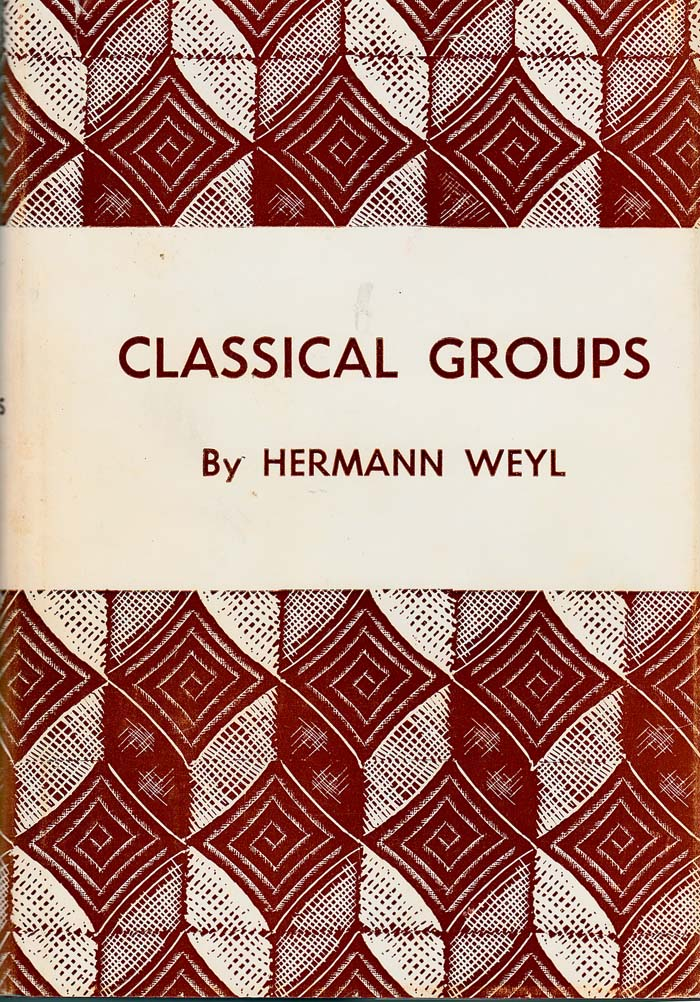
\includegraphics[width=\textwidth]{figs/weyl_classical_groups.jpg}}
		    \end{column}
	  	\end{columns}
	  	% \vfill

	  	% \hrulefill
	  	
	  	% {\tiny Recall that $\Sp_{n}(\mathbb{C})$ is defined when $n$ is even, say $n = 2m$, as the group of invertible matrices $A$ satisfying $A^{\top} \Omega A = \Omega$, where $\Omega = \left(\begin{smallmatrix} O & I_{m} \\ -I_{m} & O \end{smallmatrix}\right)$. }
	\end{frame}

	\begin{frame}{What are invariants?}
		From Fulton, Harris \cite{FultonHarris}: The goal is to find those polynomials $f(x^{(1)}, \ldots, x^{(m)})$ of $m$ variables on $V$ which are invariant by $G$. \newline

		\pause Concretely: Consider the polynomial ring $R = \mathbb{C}[X_{n \times m}]$ in $nm$ variables indexed as $x_{11}, \ldots, x_{nm}$. \pause Each $A \in G$ extends to a ring automorphism $A : R \to R$ given by $X \mapsto AX$. \newline

		\pause The question is then asking precisely what is the \deff{fixed subring}
		\begin{equation*} 
			R^{G} \vcentcolon= \{f \in R : A(f) = f \text{ for all } A \in G\}.
		\end{equation*}

		\pause This is indeed a subring. \pause A graded $\mathbb{C}$-subalgebra even. 

		\pause
		\begin{blurb} 
			If one wishes to be coordinate-free, these notions can be defined in terms of symmetric algebras, duals, and tensor products.
		\end{blurb}
	\end{frame}

	\begin{frame}{Getting our bearings straight}
		Consider $A \vcentcolon= \smatrix{1 & 1 \\ 0 & 1} \in \SL_{2}(\mathbb{C})$ and $R = \mathbb{C}[X_{2 \times 2}]$. 

		\pause Note $A \smatrix{x_{11} & x_{12} \\ x_{21} & x_{22}} = \smatrix{x_{11} + x_{21} & x_{12} + x_{22} \\ x_{21} & x_{22}}$. \pause Thus, the action of $A$ on $R$ is given by
		\begin{align*} 
			x_{11} \mapsto x_{11} + x_{21},\qquad& x_{12} \mapsto x_{12} + x_{22}, \\
			x_{21} \mapsto x_{21},\qquad& x_{22} \mapsto x_{22}.
		\end{align*}
		\pause This gives us $A(x_{11} x_{22}) = \pause A(x_{11}) A(x_{22}) = \pause (x_{11} + x_{21})x_{22}$, \pause and $A(x_{21} x_{12}) = x_{21}(x_{12} + x_{22})$. \newline

		\pause Some invariant polynomials are \pause $x_{21}$, \pause $x_{22}$, \pause $x_{21}^{43} - x_{22}^{3} x_{21}$, \pause constants, \pause and $x_{11} x_{22} - x_{21} x_{12}$.
	\end{frame}

	\begin{frame}{Invariants of \texorpdfstring{$\SL$}{SL}}
		Let $G = \SL_{n}(\mathbb{C})$ and $R = \mathbb{C}[X_{n \times m}]$. \pause Let $\{\Delta\}$ be the set of $n \times n$ minors of $X$. \pause It it okay to check that $\{\Delta\} \subset R^{G}$. \pause

		\begin{theorem}
			$R^{G} = \mathbb{C}[\{\Delta\}]$.
		\end{theorem}
		\pause
		\begin{proof}[Proof for $m < n$]
			We wish to show that the only invariants are the constants. \pause

			Suppose $f$ is invariant, and $A \in G$. \pause Then, $f(Ae_{1}, \ldots, Ae_{m}) = f(e_{1}, \ldots, e_{m})$. \pause Since $m < n$, given any linearly independent $m$-tuple $(v_{1}, \ldots, v_{m})$, there is an element $A \in \SL_{n}(\mathbb{C})$ carrying $\mathbf{e}$ to $\mathbf{v}$. \pause Thus, $f$ is constant on all $m$-tuples of linearly independent vectors. \pause By the density of such tuples, $f$ is constant, i.e., $f \in \mathbb{C} \subset R$.
		\end{proof}
	\end{frame}

	\begin{frame}{Invariants for \texorpdfstring{$\GL$}{GL}}
		Let us now consider $G = \GL_{n}(\mathbb{C})$ and $R = \mathbb{C}[X_{n \times m}]$. \pause

		For $\alpha \in \mathbb{C}^{\times}$, consider $A = \alpha I$. \pause Then, $A$ acts on $R$ by scaling the variables by $\alpha$. \pause Consequently, $A$ on a degree $d$ element $f$ by $f \mapsto \alpha^{d} f$. \pause

		\begin{corollary}
			$R^{G} = \mathbb{C}$.
		\end{corollary}

		\pause Note: This would work for any infinite field.
	\end{frame}

	\begin{frame}{Invariants for \texorpdfstring{$\GL$}{GL}: take two}
		The more interesting action for $G = \GL_{n}(\mathbb{C})$ turns out to be on the polynomial ring $R = \mathbb{C}[Y_{p \times n}, Z_{n \times q}]$. \pause $A \in G$ acts on $R$ via
		\begin{align*} 
			Y &\mapsto Y A^{-1}, \\
			Z &\mapsto AZ.
		\end{align*}

		\pause 
		Symbolically, the action of $A$ on $YZ$ would be given as
		\begin{equation*} 
			YZ \mapsto \pause (Y A^{-1}) (AZ) \pause = Y (A^{-1} A) Z = \pause YZ.
		\end{equation*}
		\pause
		One checks that the $pq$ many polynomials appearing as the entries of $YZ$ are all invariant.

		\pause 
		\begin{theorem}
			$R^{G} = \mathbb{C}[YZ]$.
		\end{theorem}
	\end{frame}

	\begin{frame}{Invariants for \texorpdfstring{$\OO$}{O} and \texorpdfstring{$\Sp$}{Sp}}
		For $\OO_{n}$ and $\Sp_{n}$, we revert to our usual action of $A$ acting via $X \mapsto AX$. \pause As before, the obvious symbolically fixed elements give us all. \pause

		For example, $A \in \OO_{n}$ acts as
		\begin{equation*} 
			X^{\top} X \mapsto \pause (AX)^{\top} (AX) = \pause (X^{\top} A^{\top}) (A X) \pause = X^{\top} (A^{\top} A) X = \pause X^{\top} X.
		\end{equation*}
		\pause 

		\begin{theorem}
			$\mathbb{C}[X_{n \times m}]^{\OO_{n}} = \mathbb{C}[X^{\top} X]$ and $\mathbb{C}[X_{n \times m}]^{\Sp_{n}} = \mathbb{C}[X^{\top} \Omega X]$.
		\end{theorem}
	\end{frame}

	\begin{frame}{A Brief Word about the proofs}
		Define the following operators on $R \vcentcolon= \mathbb{C}[X_{n \times m}]$:
		\begin{equation*} 
			D_{ij} = \sum_{k = 1}^{n} x_{ki} \dfrac{\partial}{\partial x_{kj}} \quad\text{and}\quad \Omega = \det \left[\dfrac{\partial}{\partial x_{ij}}\right]_{1 \le i, j \le m}.
		\end{equation*}
		\pause 
		The \emph{Capelli identity} says that
		\begin{equation*} 
			\det 
			\begin{bmatrix}
				D_{11} + m - 1 & D_{12} & \cdots & D_{1m} \\
				D_{21} & D_{22} + m - 2 & \cdots & D_{2m} \\
				\vdots & \vdots & \ddots & \vdots \\
				D_{m1} & D_{m2} & \cdots & D_{mm}
			\end{bmatrix}
			= \det(X_{n \times m}) \cdot \Omega
		\end{equation*}
		as operators on $R$ when $n = m$. \pause

		If $F$ is an invariant of $G$, so is each $D_{ij}(F)$. Note that $D_{ij}$ lowers the $j$-th degree by $1$ while increasing the $i$-th degree by $1$. Induct...
	\end{frame}

	\begin{frame}{Non-classical?}
		If we replace $\mathbb{C}$ with an arbitrary infinite field $K$, the earlier results still hold true. \pause \hfill {\tiny Modulo some care in characteristic two.}

		\pause However, in positive characteristic, the groups are not linearly reductive \pause ($\approx$ semisimple). 

		\pause In particular, in characteristic zero, the inclusion
		\begin{equation*} 
			R^{G} \subset R
		\end{equation*}
		splits (as $R^{G}$-modules) when $G$ is a classical group with the natural action. 

		\pause This is similar to the finite group case when we have a splitting given by $r \mapsto \frac{1}{\md{G}} \sum\limits_{g \in G} g(r)$.
	\end{frame}

	% \begin{frame}{When do they split in positive characteristic?}
	% 	\begin{theorem}
	% 		Let $K$ be a field of characteristic $p > 0$. Let $A \subset R$ denote one of the following inclusions:
	% 		\begin{enumerate}[label=(\alph*)]
	% 			\item $K[YZ] \subset K[Y_{p \times n}, Z_{n \times q}]$;
	% 			\item $K[X^{\top} \Omega X] \subset K[X_{2n \times m}]$;
	% 			\item $K[X^{\top} X] \subset K[X_{n \times m}]$;
	% 			\item $K[\{\Delta\}] \subset K[X_{n \times m}]$.
	% 		\end{enumerate}
	% 		The inclusion splits if and only if, in the respective cases,
	% 		\begin{enumerate}[label=(\alph*)]
	% 			\item $n = 1$ or $\min\{m, n\} \le t$;
	% 			\item $m \le n + 1$;
	% 			\item $n = 1$; $n = 2$ and $p$ is odd; $p = 2$ and $m \le (n + 1)/2$; or $p$ is odd and $m \le (n + 2)/2$;
	% 			\item $n = 1$ or $n = m$.
	% 		\end{enumerate}
	% 	\end{theorem}
	% \end{frame}

	\begin{frame}{When do they split in positive characteristic?}
		The following is from \cite{HochsterJeffriesPandeySingh}. \pause

		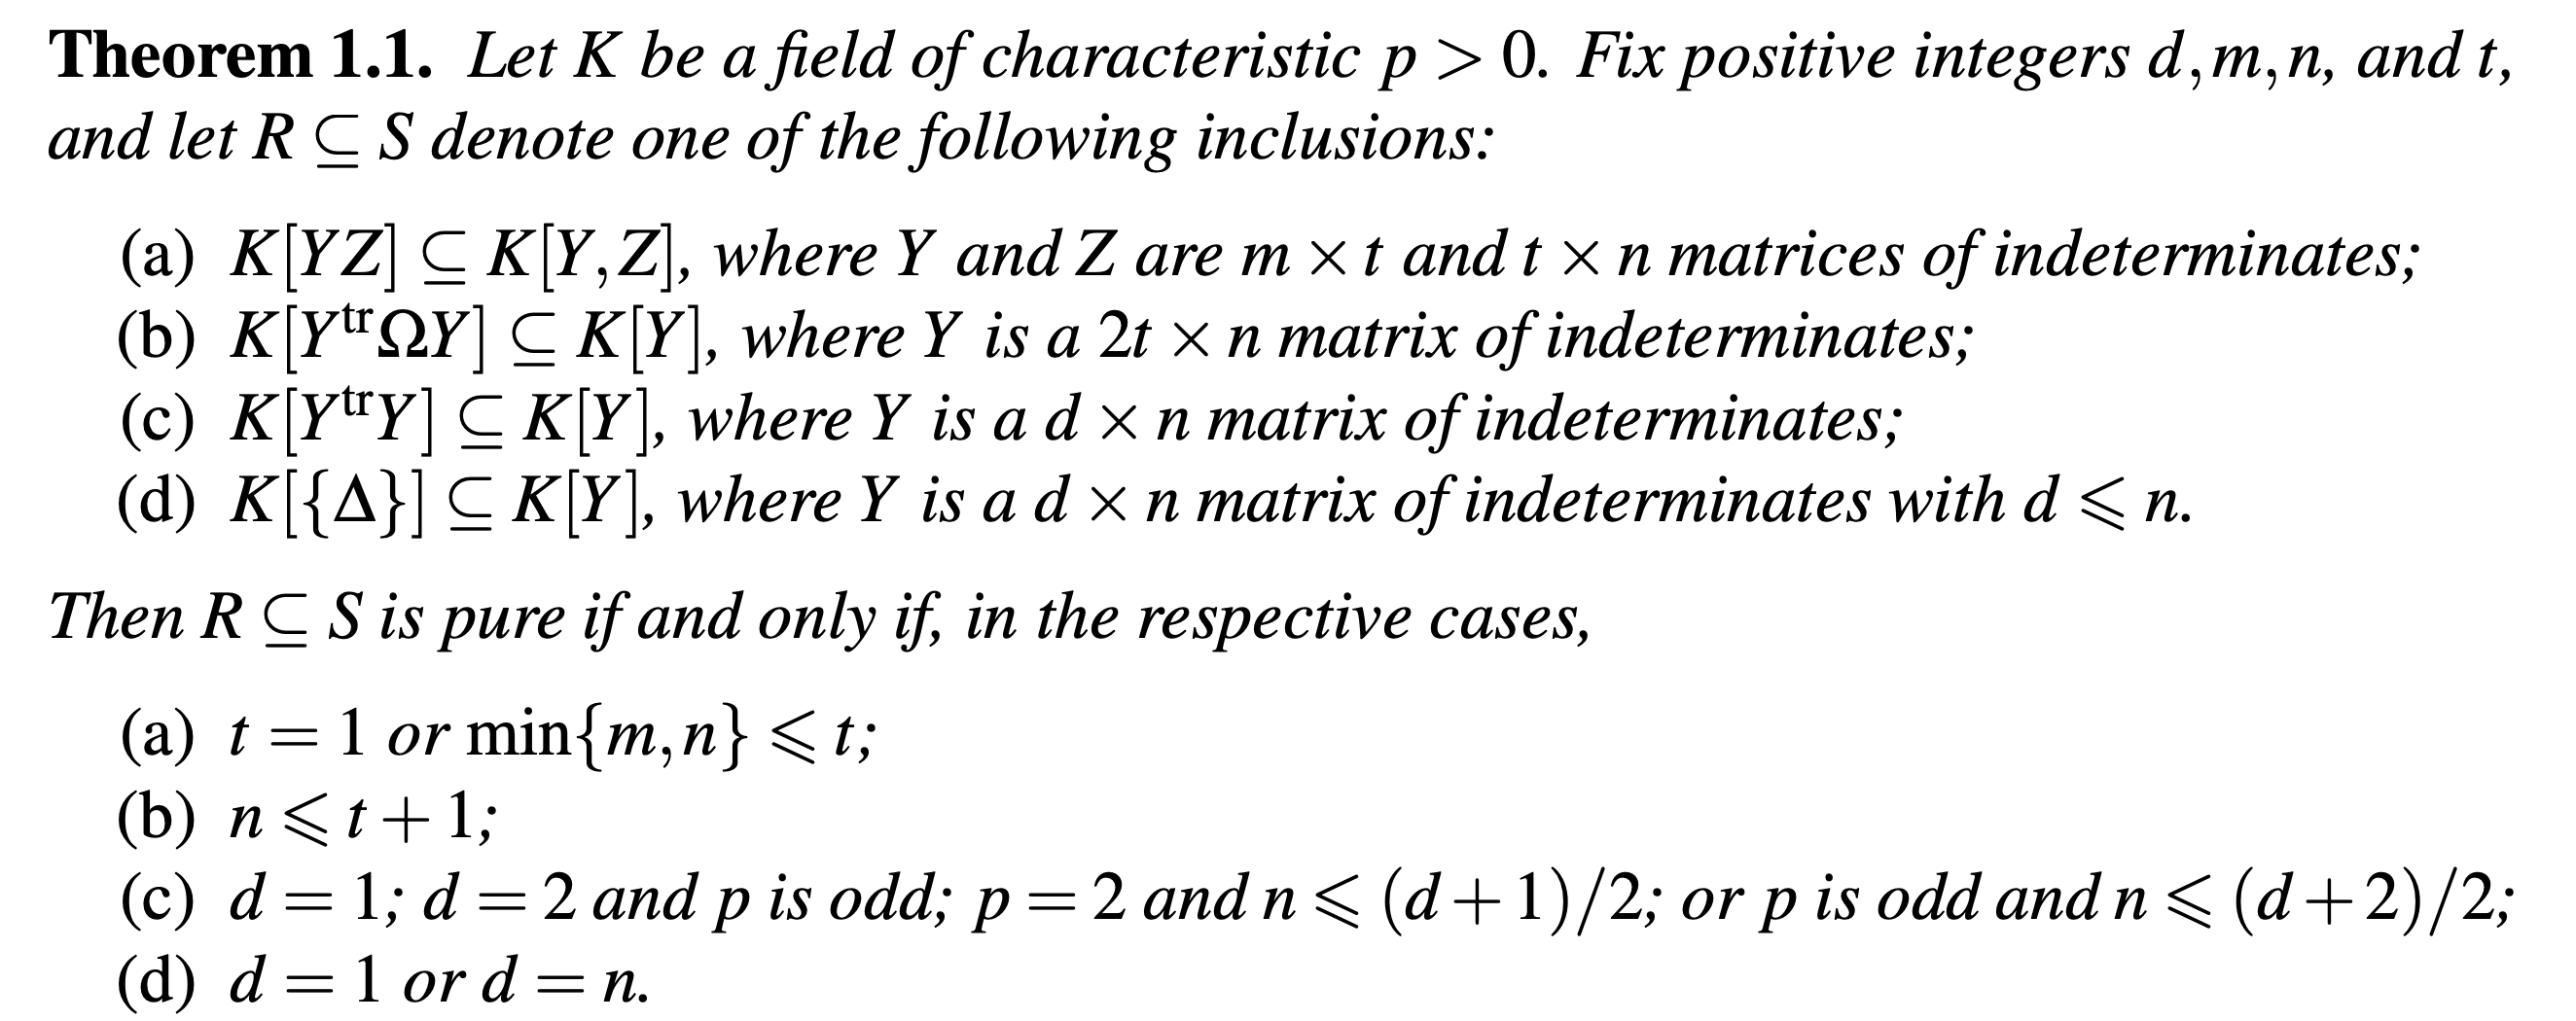
\includegraphics[width=\textwidth]{figs/HJPS_main_theorem.png}

		These cases are essentially the ``obvious'' ones: in these cases, either the subring $R$ is regular, or the corresponding group was linearly reductive. \pause 
		\begin{blurb}
			Note that the above theorem applies even if $K$ is finite; however, the subring does not arise from the corresponding group action in those cases.
		\end{blurb}
	\end{frame}

	\begin{frame}{What does this mean?}
		Concretely: let us consider the inclusion $R \subset S$ where $S = \mathbb{Q}[X_{2 \times 3}]$ and $R = \mathbb{Q}[\Delta_{1}, \Delta_{2}, \Delta_{3}]$ is the subring generated by the three $2 \times 2$ minors of $X$. \pause

		As an $R$-module, $S$ has a generating set consisting of all the monomials. \pause Since we are in char zero, we have a splitting $f : S \to R$. \pause However, for every prime $p$, the map $\mathbb{F}_{p}[\{\Delta\}] \subset \mathbb{F}_{p}[X_{2 \times 3}]$ does \emph{not} split. 

		\pause What this means is that for every prime $p$, there is some monomial $m_{p} \in S$ such that the expression for $f(m_{p})$ in terms of the $\Delta_{i}$ has a $p$ in the denominator.
	\end{frame}

	\begin{frame}{Finite fields?}
		\begin{block}{Natural question}
			What are the invariant subrings when $K = \mathbb{F}_{p}$? Do they split?
		\end{block}
		Even the first action of $\GL_{n}(K)$ on $K[X_{n \times m}]$ is not trivial now. \pause In the case that $m = 1$, the fixed subring is generated by the $n$ algebraically independent \emph{Dickson invariants}. 
	\end{frame}

	\begin{frame}{Fin}

		\vfill 

		Thank you for your attention!

		\vfill
	\end{frame}

	\begin{frame}{References}
		\printbibliography
	\end{frame}
\end{document}